\section{五级流水线：从结构图到 RTL}
\label{sec:04-processor-core-04}

\subsection{先把一条指令的工作分开，再让多条指令重叠}

单周期处理器把取指、译码、读寄存器、运算、访存和写回串在一个时钟周期内。
画数据通路时，我们很容易沿着箭头说出一条指令走过哪些部件；开始写 RTL 时，
更重要的问题却是：\textbf{哪些信号只是当前时刻的组合结果，哪些信号必须保存到下一拍？}
五级流水线正是围绕这个问题重新安排状态边界。

本节以第 4.02 节的单周期思想为起点，把一条指令的处理划分为
IF（取指）、ID（译码与读寄存器）、EX（执行）、MEM（访存）和 WB（写回）。
相邻阶段之间加入流水寄存器，保存该条指令后面还要使用的数据和控制信息。
划分完成后，同一周期内可以同时有五条不同的指令分别占据五个阶段。
每一级中的组合电路并行工作，在同一个上升沿把结果交给下一级。

本节结束时，读者应当能够从结构图中圈出状态元件，把跨级信号整理成字段表，
并解释一个时钟边沿上四组流水寄存器为什么同时更新却不会让指令一下穿过四级。
第 4.05 节继续解决重叠执行带来的数据相关和控制相关。
读者应先完成\cref{sec:02-digital-logic-04}的模块、组合逻辑和时序逻辑练习。
这里沿用前文“先想电路、再写代码”的方法，不重复 Verilog 基础语法，也不把实验扩展成一颗完整 CPU。

\KeyPoint{本实验的明确边界}{
数据宽度为 32 位，顺序、单发射、五级流水；只实现 ADD、SUB、ADDI、LW、SW 和 BEQ。
不包含异常、中断、CSR、Cache、乘除法、总线等待、字节访存和完整 RV32I 合规性。
因此文中的“教学数据通路”不能直接标记为完整 RV32I 处理器。}

\subsection{先写时序合同，才能判断结构图是否正确}

流水线的分级是一种微架构选择，指令集并不规定必须采用五级结构。
RV32I 规定寄存器、指令编码和可见效果，例如 x0 恒为零、LW 按有效地址取一个字、
BEQ 比较两个寄存器并使用相对当前指令 PC 的分支偏移\cite{ch4-rv32i}。
指令在哪一级读寄存器、存储器何时返回数据、分支在哪一级决策，则必须由实现者说明。
本实验采用\cref{tab:ch4-contract} 的时序合同，后面的暂停次数和波形均在这些条件下成立。

\begin{table}[htbp]
\centering\small
\caption{教学数据通路的时序合同}\label{tab:ch4-contract}
\begin{tabularx}{\linewidth}{p{.22\linewidth}Y}
\toprule
项目 & 本实验的约定 \\\midrule
时钟与复位 & 上升沿触发；高电平同步复位。仿真周期为 10 ns。\\
取指接口 & 独立指令存储器，组合读；PC 稳定后，本周期内得到指令。\\
数据接口 & 独立数据存储器，组合读、上升沿写；只接受对齐的 32 位字访问。\\
寄存器堆 & 两个组合读端口、一个上升沿写端口；显式提供 WB 到 ID 的同拍旁路。\\
分支 & BEQ 在 EX 比较并计算目标；默认顺序取指，分支成立时重定向。\\
完成时间 & ALU 结果在 EX 结束时可供后续级使用；load 数据在 MEM 结束时可供后续级使用。\\
结构资源 & 指令存储器与数据存储器分离，本实验不产生二者争用同一端口的结构冒险。\\
\bottomrule
\end{tabularx}
\end{table}

这里的组合读存储器是为了把注意力集中在流水线控制。
FPGA 的同步块 RAM 通常要求先在时钟边沿采样地址，再输出数据；AXI 和 Cache 还可能插入不定长等待。
因此不能把本例的数组简单替换成这些资源，就继续沿用“load-use 总是停一拍”的结论。
接入 SoC 时，应先核对请求何时被接受、响应何时有效，以及等待期间哪些流水级需要保持。
更一般的 ready/valid 背压协议属于接口扩展，不在本例的固定延迟模型内。

\subsection{三种结构，三种 RTL 阅读方法}

\begin{figure}[htbp]
\centering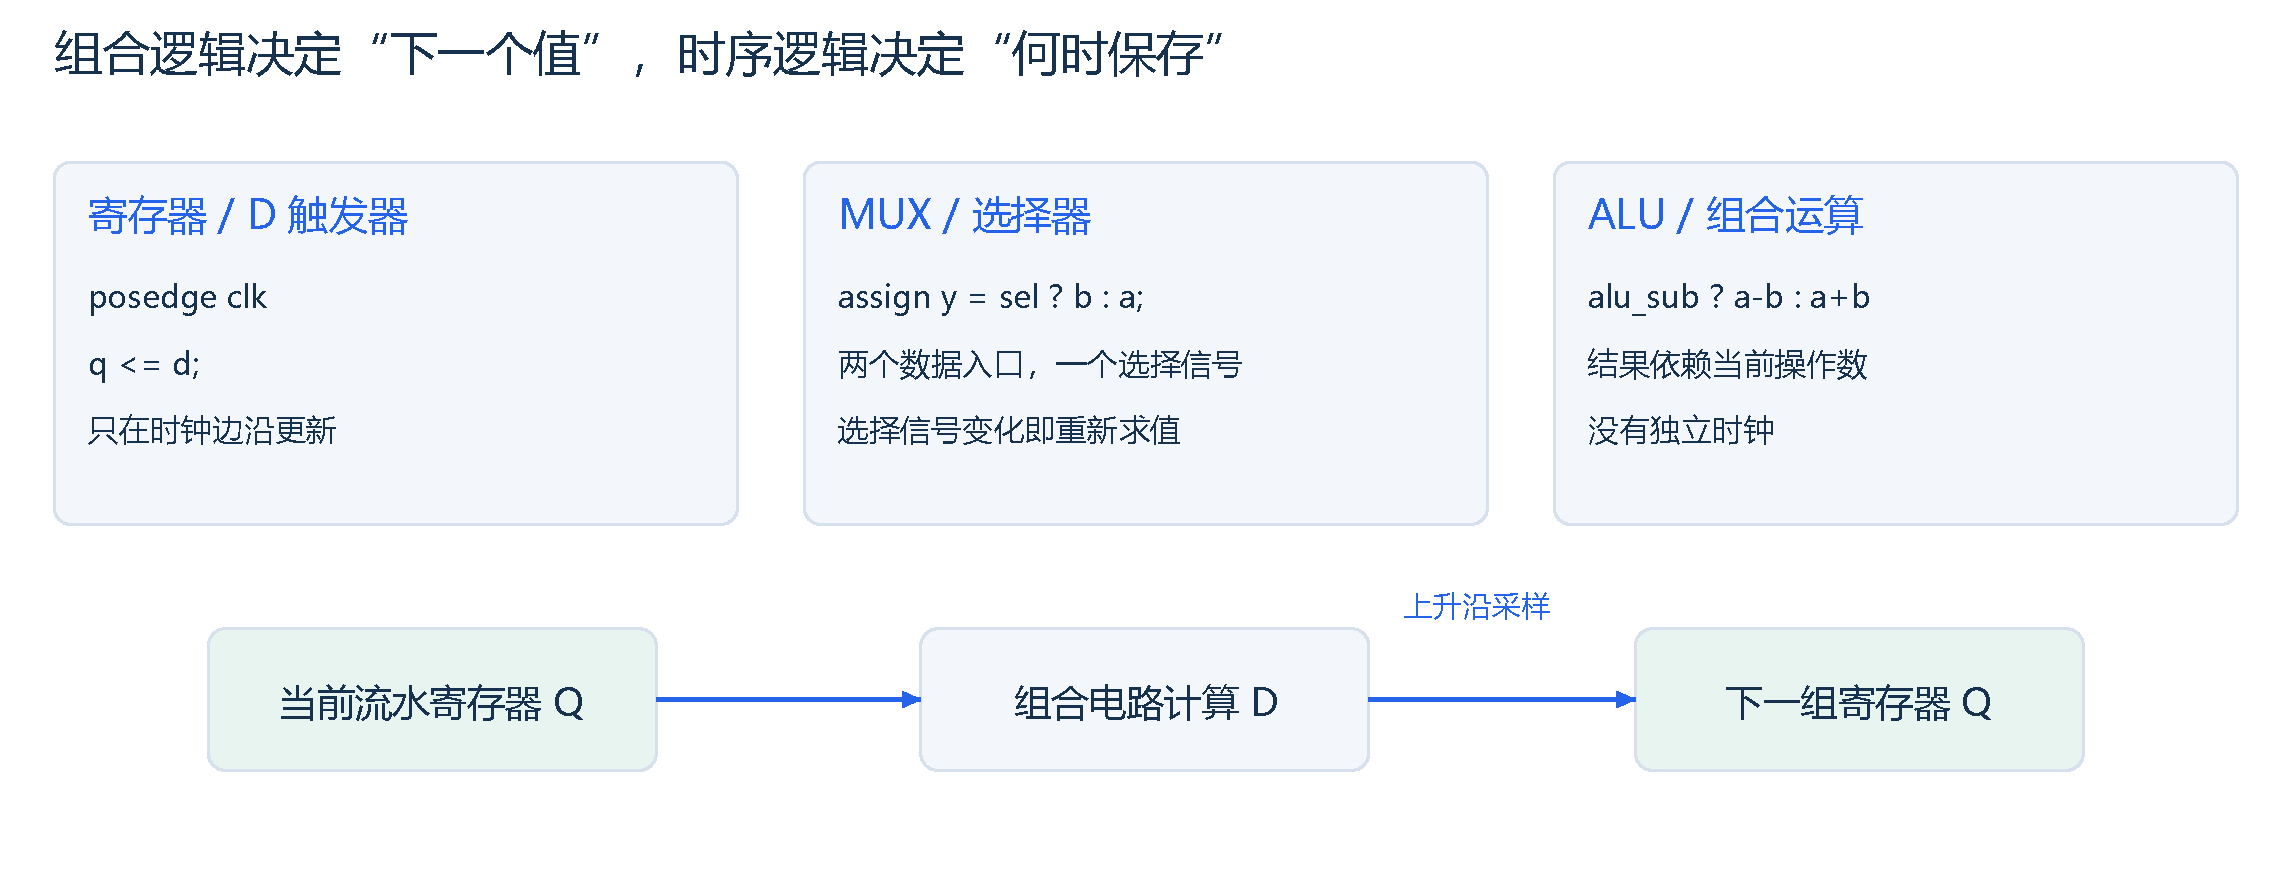
\includegraphics[width=\linewidth]{figures/04-pipeline/rtl-mapping}
\caption{组合逻辑与时序状态的对应关系。图形由代码生成，SVG 与 PDF 使用同一组几何元素。}
\label{fig:ch4-mapping}
\end{figure}

\paragraph{寄存器保存跨周期的状态。}
结构图中的寄存器不是一根被命名的数据线，而是保存旧值的状态元件。
\texttt{always @(posedge clk)} 中的非阻塞赋值描述上升沿采样。
若某个分支没有对寄存器赋值，该寄存器保留原值；这正是时钟使能的行为。
代码中的 \texttt{reg} 只是一种 Verilog 变量类型，是否综合成触发器要看赋值所在的过程，不能仅凭声明判断。

\paragraph{MUX 选择当前要使用的输入。}
\texttt{assign y = sel ? b : a;} 表示二选一组合电路。
在流水线里，PC 选择器决定顺序地址还是分支目标，ALU 输入选择器决定寄存器值还是立即数，
WB 选择器决定 ALU 结果还是载入数据。
选择器本身不使指令“进入下一拍”；只有结果被寄存器采样，状态才发生推进。

\paragraph{ALU 根据输入持续计算。}
加法和减法可直接用运算符表达。本实验使用一个控制位 \texttt{alu\_sub} 选择加减。
综合器可以据此实现共享的加减电路，具体门级实现由综合优化决定。
组合逻辑中的默认赋值则保证每条路径都有确定输出，避免无意引入锁存器。

\begin{table}[htbp]
\centering\small
\caption{从结构图到代码时应追问什么}\label{tab:ch4-rtl-map}
\begin{tabularx}{\linewidth}{p{.18\linewidth}p{.28\linewidth}Y}
\toprule
图上的部件 & 本例代码形式 & 阅读时的关键问题 \\\midrule
PC 寄存器 & 上升沿过程 + 使能 & 复位、重定向、暂停、顺序推进，谁的优先级更高？\\
流水寄存器 & 一组非阻塞赋值 & 数据、目的寄存器号和控制信号是否属于同一条指令？\\
译码器 & 完整默认值 + case & 这条指令真正读取哪些源寄存器，后面需要哪些控制？\\
寄存器堆 & 数组 + 双组合读 + 单时序写 & x0 是否保持零；WB 和 ID 同拍访问同一地址时得到什么？\\
MUX / ALU & 连续赋值或组合过程 & 选择条件来自哪一级；输入是旧读值还是前递后的新值？\\
存储器写口 & 地址、数据、写使能 & 写使能是否受有效位控制，错误路径能否造成写入？\\
\bottomrule
\end{tabularx}
\end{table}

\subsection{把数据通路切成五级}

\begin{figure}[htbp]
\centering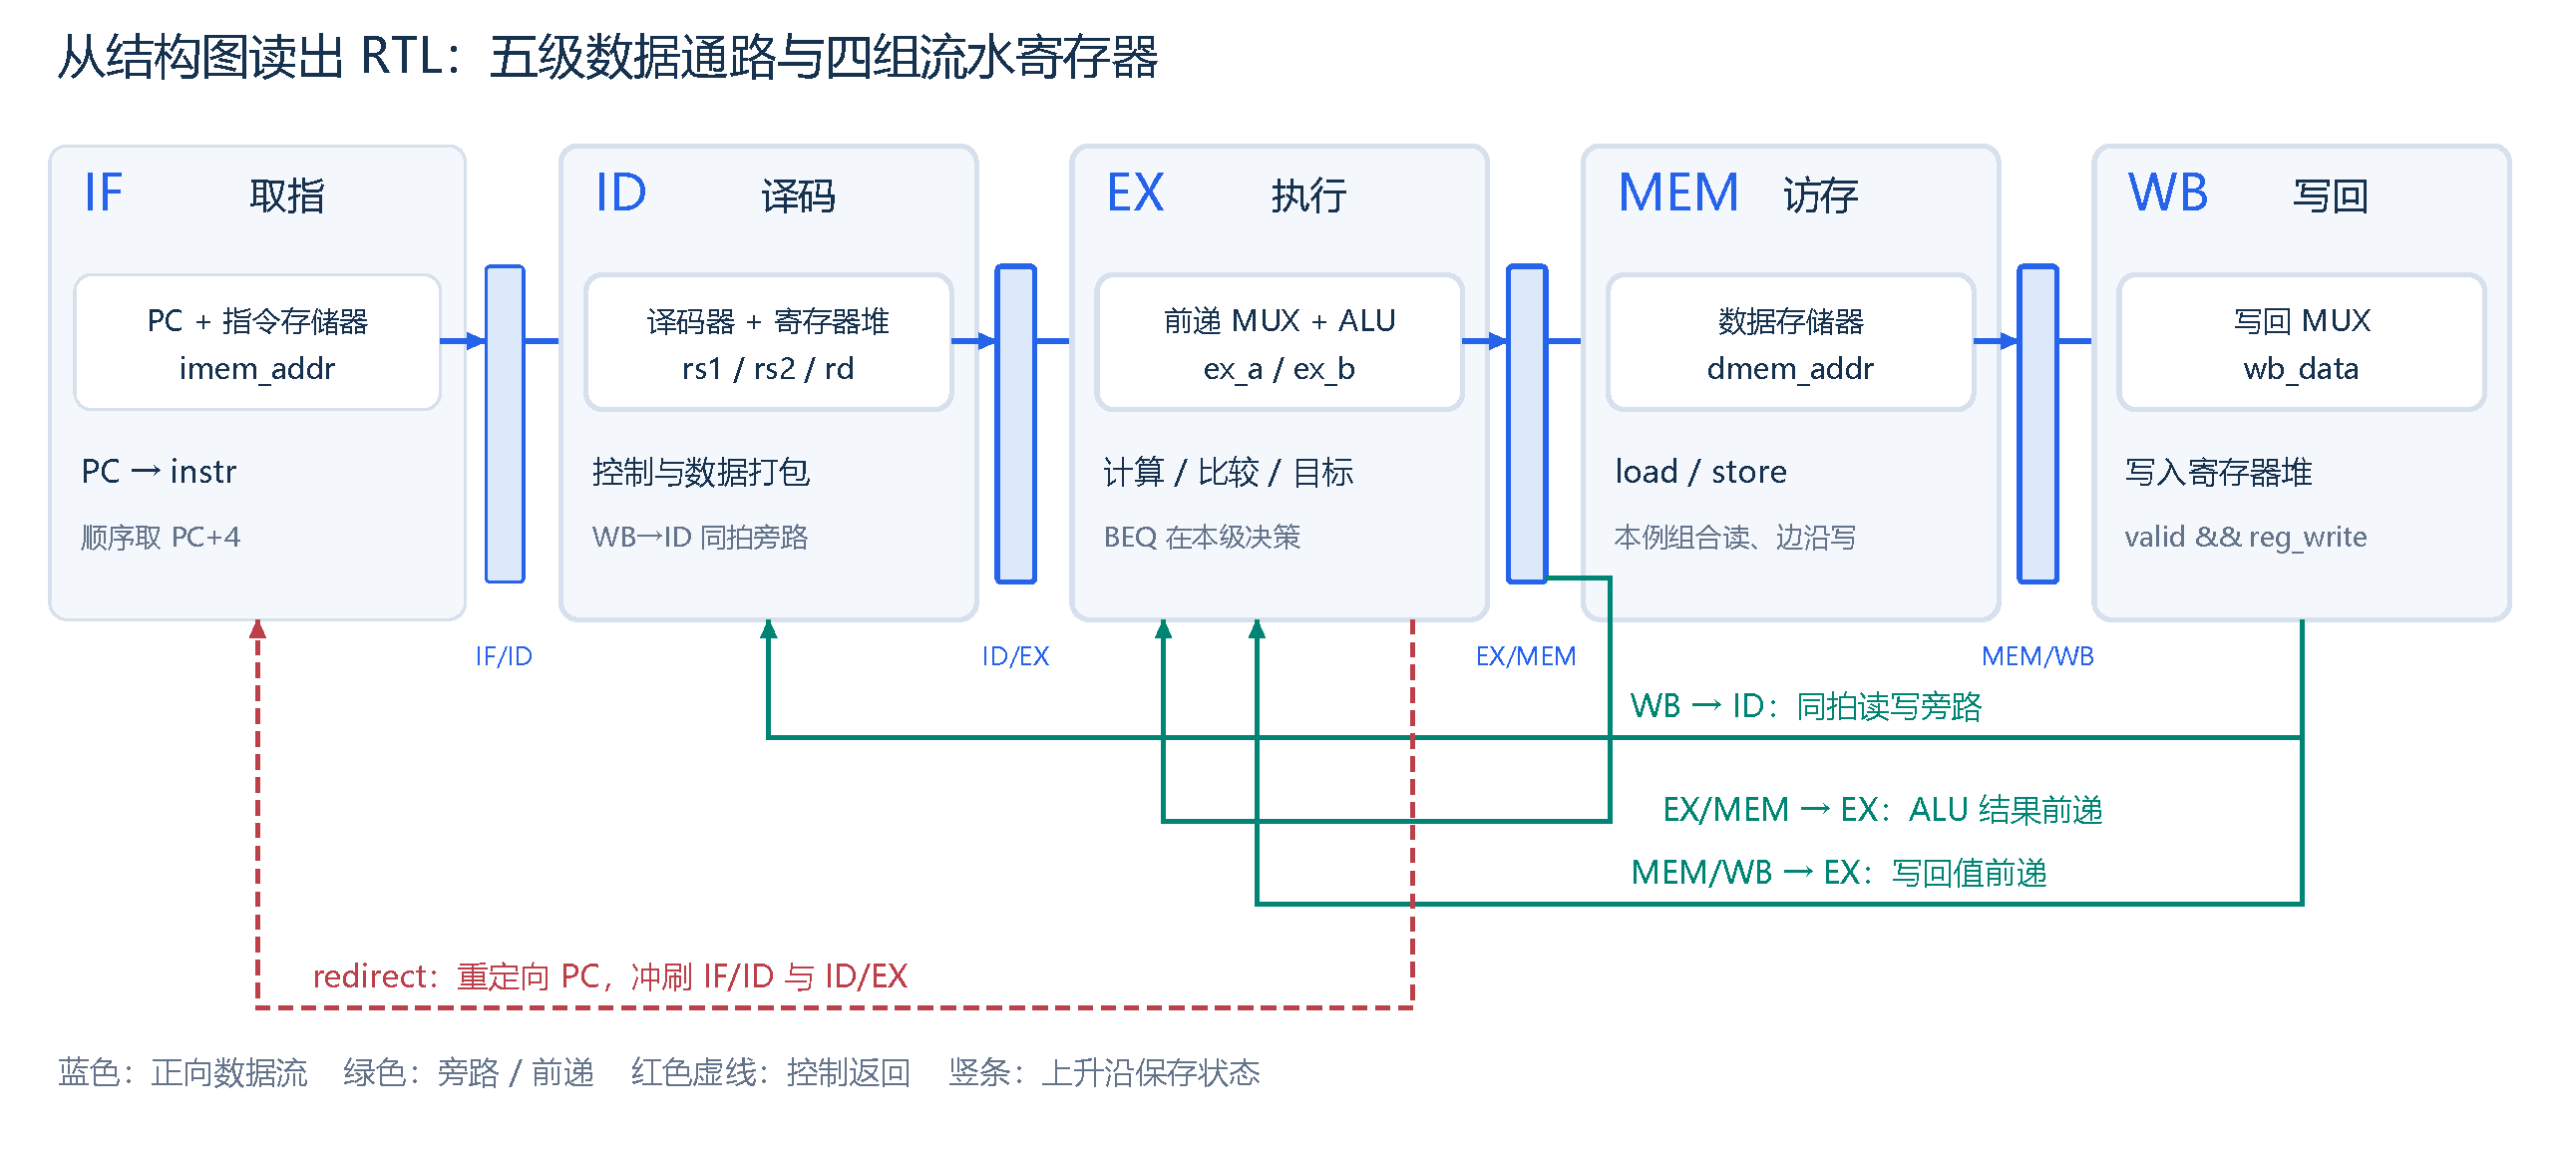
\includegraphics[width=\linewidth]{figures/04-pipeline/rtl-datapath}
\caption{五级数据通路的主要数据流和控制返回路径。竖条表示流水寄存器；图中省略了部分逐位连线。}
\label{fig:ch4-datapath}
\end{figure}

IF 用当前 PC 访问指令存储器，把取回的指令和该指令的 PC 交给 IF/ID。
ID 解析指令、读取寄存器并形成立即数，把执行所需的信息交给 ID/EX。
EX 计算算术结果或访存有效地址；BEQ 也在这里比较，并计算目标地址。
MEM 对 load 读取数据、对 store 写入数据。非访存指令在这一阶段只传递结果。
WB 在 ALU 结果与载入数据之间选择，更新目的寄存器。

以 \texttt{lw x4, 0(x0)} 为例，EX 做的是 \(0+0\) 的地址计算，MEM 才读取地址 0 对应的数据，
WB 再写 x4。以 \texttt{sw x3, 0(x0)} 为例，EX 同样计算地址，但还必须把 x3 的值保存到 EX/MEM，
MEM 才能用它作为写数据。\textbf{地址和写数据是两条不同的路径。}
store 不写通用寄存器，它的 \texttt{reg\_write} 必须为 0。

\paragraph{增加流水级不等于单条指令更快。}
若各级组合延迟为 \(t_i\)，流水寄存器开销为 \(t_r\)，时钟周期需满足
\(T_{\mathrm{clk}}\geq\max_i(t_i)+t_r\)。理想情况下，\(N\) 条指令经过五级流水需要
\(N+4\) 个周期；单条指令仍然要跨过五级。
举一个只用于理解的数值例子：单周期组合路径为 10 ns，五级各为 2 ns，寄存器开销为 0.2 ns。
单条指令的流水延迟为 11 ns，但长指令流的完成间隔可接近 2.2 ns。
这些数字不是本工程的综合测量结果；本实验只验证功能与周期行为，不报告可达到的 FPGA 主频。

\subsection{流水寄存器保存的是“一条指令的上下文”}

最常见的错误是只保存计算数据，却让控制信号直接使用 ID 当前译出的结果。
当一条 load 已经进入 MEM 时，ID 中可能是一条 add。若 MEM 仍使用当前 ID 的 \texttt{mem\_read}，
访存行为就由另一条指令控制了。因此，控制信号也必须逐级寄存。
\cref{tab:ch4-fields} 给出本例实际字段与后续用途，读者可以逐项与
\texttt{pipeline\_demo.v} 的声明对应。

\begin{table}[htbp]
\centering\small
\caption{四组流水寄存器中的内容}\label{tab:ch4-fields}
\begin{tabularx}{\linewidth}{p{.15\linewidth}p{.40\linewidth}Y}
\toprule
边界 & 字段类别 & 下一阶段为什么需要它 \\\midrule
IF/ID & valid、pc、instr & ID 需要机器指令，分支后续需要原始 PC。\\
ID/EX & valid、pc、rv1/rv2、rs1/rs2、rd、imm；use1/use2、rw、mr、mw、ai、sub、br & EX 使用操作数、立即数和 ALU/分支控制；源寄存器号供前递比较，后级控制继续随指令传递。\\
EX/MEM & valid、pc、result、store、rd；rw、mr、mw & result 是 ALU 结果或有效地址，store 是前递后的写数据，MEM 据 mr/mw 执行访存。\\
MEM/WB & valid、pc、result、load、rd；rw、mr & mr 选择写回值，rd 指定写入对象，rw 指定是否写回。\\
\bottomrule
\end{tabularx}
\end{table}

其中缩写 \texttt{rw/mr/mw} 分别表示寄存器写、存储器读和存储器写，
\texttt{ai/sub/br} 分别表示 ALU 使用立即数、减法和分支。
为了便于波形定位，PC 在本例中一直传到 WB；它不是每一种最小数据通路都必须保留到最后的功能字段。
同样，\texttt{commit\_pc} 等输出是观察接口，用来核对写回，不代表已经实现了处理器的异常提交机制。

\paragraph{valid 决定这一格是否装着有效指令。}
当 \texttt{valid=0} 时，其他字段可以保留旧数据。
寄存器写、存储器写、分支重定向和冒险检测都必须检查相应的 valid。
这样只清有效位就能让空泡失去所有副作用，无需把整组数据清零。
这也解释了仿真中为何可能看见无效级内存在旧地址、旧目的寄存器号甚至 X：
判断电路是否执行了操作，必须同时看有效位和使能，不能孤立地读一条数据总线。

\paragraph{一次上升沿只前进一级。}
假设边沿前 ID/EX 保存指令 A，EX/MEM 保存指令 B。
边沿到来时，EX/MEM 接收由 A 计算出的结果，同时 MEM/WB 接收 B 的访存或运算结果。
非阻塞赋值的右值在更新前求值，再统一更新目标寄存器，
因此 MEM/WB 不会在同一个边沿接收到刚更新进 EX/MEM 的 A。
把这些过程按源文件从上往下理解成软件执行顺序，会得出错误的流水线行为。

\par\noindent\begin{minipage}{\linewidth}\vspace{8pt}
\lstinputlisting[language=Verilog,caption={PC、IF/ID 与 ID/EX 的实际更新逻辑},label={lst:ch4-registers}]{code/04-pipeline/listings/pipeline-registers.v}
\end{minipage}\par

代码中的 \texttt{ifid\_en=0} 使 IF/ID 保持，而 \texttt{idex\_flush=1} 使下一拍 EX 为空泡。
二者作用对象不同，不能笼统地替换为“全流水暂停”。
后级在这种情况下仍继续推进，如\cref{lst:ch4-late} 所示。

\par\noindent\begin{minipage}{\linewidth}\vspace{8pt}
\lstinputlisting[language=Verilog,caption={EX/MEM 与 MEM/WB 继续接收旧指令的结果},label={lst:ch4-late}]{code/04-pipeline/listings/late-stages.v}
\end{minipage}\par

\subsection{译码的任务是产生电路需要的控制，不只是辨认名字}

本例保留了少量真实 RISC-V 指令编码，使汇编、机器码和 RTL 能逐一对照。
\cref{tab:ch4-decode} 中的控制不是所有 CPU 通用的标准接口，而是这套数据通路需要的内部信号。
完整译码位于 \texttt{decoder.v}；不支持的编码令 \texttt{legal=0}，
测试平台见到有效的非法指令会停止仿真。这是教学范围检查，不能替代真正的非法指令异常。

\begin{table}[htbp]
\centering\small
\caption{本例指令与控制信号的对应关系；1 表示启用}\label{tab:ch4-decode}
\begin{tabular}{lcccccccc}
\toprule
指令 & use1 & use2 & rw & mr & mw & ai & sub & br \\\midrule
ADD  &1&1&1&0&0&0&0&0\\
SUB  &1&1&1&0&0&0&1&0\\
ADDI &1&0&1&0&0&1&0&0\\
LW   &1&0&1&1&0&1&0&0\\
SW   &1&1&0&0&1&1&0&0\\
BEQ  &1&1&0&0&0&0&0&1\\
\bottomrule
\end{tabular}
\end{table}

\texttt{uses\_rs1} 和 \texttt{uses\_rs2} 尤其值得注意。
ADDI 的指令位 \texttt{[24:20]} 是立即数的一部分，不是第二源寄存器。
虽然代码总能从这些位切出一个数作为 \texttt{rs2}，它并不意味着这条指令真的读取了那个寄存器。
冒险检测只有在 use 位为 1 时才比较对应地址，才能避免误暂停。

立即数也属于数据通路。I 型立即数由 \texttt{instr[31:20]} 符号扩展；
S 型要把 \texttt{instr[31:25]} 与 \texttt{instr[11:7]} 拼接后符号扩展；
B 型要重排离散字段并补最低位零。
BEQ 的目标用 \texttt{idex\_pc + idex\_imm} 计算，而不能用当前 IF 的 PC，
因为决定分支时 IF 已经在读取更年轻的指令。

\subsection{寄存器堆的同拍读写必须说清楚}

本实验的寄存器堆在上升沿写入，在组合路径上读取。
x0 读口直接返回零，写口丢弃对 x0 的写入。
为了使仿真与不同物理实现之间的行为一致，当 WB 正在写入 ID 所读取的地址时，
组合读口直接选择 WB 的写数据。这条 WB 到 ID 的旁路与下一节的 WB 到 EX 前递不是同一件事。

\par\noindent\begin{minipage}{\linewidth}\vspace{8pt}
\lstinputlisting[language=Verilog,caption={双读单写寄存器堆与显式 WB 到 ID 旁路}]{code/04-pipeline/regfile.v}
\end{minipage}\par

为什么需要这条路径？设生产者在 WB、消费者在 ID。
在同一上升沿，寄存器堆的数组和消费者的 ID/EX 都发生非阻塞赋值。
若消费者在边沿前看到的是数组旧值，就可能把旧值带入 EX；等到下一周期，生产者又已经离开 MEM/WB，
EX 的前递网络也无法再从它取得数据。显式旁路让 ID 在该边沿前就看到正确的新值，消除了这个约定空白。

复位清零整个寄存器数组是为了让教学波形与测试初值可重复，并不是 RISC-V 对所有通用寄存器复位值的要求。
真实 FPGA 实现还要考虑资源推断、复位扇出和存储器原语的限制。
本例不据此给出资源占用或时序收敛结论。

\subsection{先运行一个能逐拍追踪的程序}

下面的贯穿程序既包含算术结果前递，也包含 store 数据前递、load-use 相关和 taken branch。
左列是字节地址，中列是仿真真正载入的机器码，右列是对应汇编。
\texttt{run.py} 生成这三者，因此读者可以直接回到 \texttt{program.hex} 核对实验输入。

\par\noindent\begin{minipage}{\linewidth}\vspace{8pt}
\lstinputlisting[language={},caption={贯穿两个小节的仿真程序},label={lst:ch4-program}]{code/04-pipeline/listings/walkthrough.txt}
\end{minipage}\par

顺序执行的预期结果是：x1=5，x2=10，x3=5，地址 0 写入 5；
随后 x4 从地址 0 载入 5，x5=15，x6=15。
地址 \texttt{0x1c} 的 BEQ 成立，跳到 \texttt{0x28}，因此 x7 保持复位值 0，
地址 4 保持测试平台初值 32，x8=30，地址 8 最后写入 30。
“地址 4 保持 32”比“没有看到一次异常写入”更容易做成自动判定。

\subsection{实验入口与文件之间的关系}

实验的最低要求是一台能运行 Python 和 Icarus Verilog 的电脑，不需要 FPGA 开发板。
Python 负责生成输入、执行独立的顺序指令模型和比对结果；
Icarus Verilog 实际执行 RTL 与测试平台并输出 VCD\cite{ch4-iverilog}。
仅凭 Python 的参考结果不能证明 RTL 正确，必须完成两者的比较。

在仓库根目录运行：
\begin{quote}\ttfamily\small
python chapters/04-processor-core/code/04-pipeline/run.py
\end{quote}
命令默认使用 PATH 中的 \texttt{iverilog} 与 \texttt{vvp}。
核内文件是 Verilog-2001，测试平台使用少量 SystemVerilog 功能，所以联合编译选择 \texttt{-g2012}。
核心模块另通过了 \texttt{-g2001} 语法检查；本稿记录的通过结果均来自 Icarus。

所有生成的运行产物位于 \texttt{build/rtl-pipeline/}。
每个案例都有机器码、汇编对照、\texttt{trace.csv}、\texttt{events.csv}、\texttt{wave.vcd} 和仿真日志。
前者记录周期状态，后者记录真实发生的寄存器写回和存储器写入；VCD 可以在 GTKWave 中逐信号观察。
图解网页 \texttt{code/04-pipeline/index.html} 可以直接用浏览器打开，拖动周期滑块查看五级中的指令。

\subsection{第一次运行：先确认输入，再检查输出}

\begin{enumerate}
\item 在终端运行 \texttt{python --version}、\texttt{iverilog -V} 和 \texttt{vvp -V}，
确认 Python 与仿真器已经能被找到。仅浏览配套网页不需要安装这些工具。
\item 在仓库根目录执行上一小节的 \texttt{run.py} 命令。
脚本先编译五个硬件模块和测试平台，然后分别运行八个案例。
\item 终端中每个案例应显示 \texttt{"status": "PASS"}，最后显示
\texttt{PASS: 8 programs}。这意味着寄存器写回、存储器写入和本例指定的周期约束都通过了检查；
仅生成 VCD 文件并不代表测试通过。
\item 打开 \texttt{build/rtl-pipeline/walkthrough/program.txt}，先核对地址与汇编；
再打开同目录的 \texttt{events.csv}，确认地址 0 写入 5、地址 8 写入 30，且没有地址 4 的写入。
\item 最后打开 \texttt{wave.vcd} 或网页逐拍演示，从 C4、C7、C11 三个关键点观察数据从哪里来。
先明确要验证的事件，再选择信号，比一次加入全部信号更容易理解。
\end{enumerate}

\begin{table}[htbp]
\centering\small
\caption{首次复现实验时的定位顺序}\label{tab:ch4-first-run}
\begin{tabularx}{\linewidth}{p{.29\linewidth}Y}
\toprule
现象 & 先检查什么 \\\midrule
找不到 iverilog 或 vvp & 确认仿真器已安装，并将其可执行文件目录加入 PATH。\\
编译出现重复模块 & 只编译五个完整模块与测试平台，不把 \texttt{listings/} 的教材摘录重复加入。\\
能生成波形，但脚本报错 & 阅读失败案例的 \texttt{simulation.log}，再比较 \texttt{events.csv}；不要忽略非零退出状态。\\
波形比教材“早一拍” & 检查游标在上升沿之前还是之后；本文按边沿前、NBA 更新前采样。\\
无效级内出现 X & 同时检查该级 valid 与副作用使能；本例只复位有效位，不清空所有载荷。\\
\bottomrule
\end{tabularx}
\end{table}

\KeyPoint{阅读 RTL 的顺序}{
先读接口时序合同，再读流水寄存器字段；随后沿一条指令追踪数据和控制，最后加入前递、暂停与冲刷。
先弄清每个信号属于哪一条指令、哪一个周期，比先背诵控制信号名称更有用。}

\subsection{小结与思考}

本节把结构图中的寄存器、选择器、运算器和连线映射成实际 RTL。
流水线的关键新增状态是四组流水寄存器；它们不仅传递数据，也传递控制和有效位。
下一节将看到，只要结果就绪时间与使用时间不一致，普通的逐级传递就需要前递或暂停配合。

\begin{enumerate}
\item 如果把 MEM 的写使能直接连接到 ID 的 \texttt{d\_mw}，哪两条不同年龄的指令会被混在一起？
\item 若一组流水寄存器的 valid 为 0，但数据中仍有非零数值，是否必须清零数据才能保证正确？请列出需要门控的副作用。
\item 若将组合读数据存储器改成同步读 BRAM，应该先检查哪一条时序合同，而不是直接修改暂停计数？
\item 在 WB 与 ID 同拍使用 x1 的情况下，为什么寄存器堆使用非阻塞写并不足以保证 ID 获得新值？
\end{enumerate}
